% 1) Title
% 2) Date
% 3) Location
% 4) Present
% 5) Picture
% 6) Start Time
% 7) Stop Time
\insertmeeting 
	{Team Takeover} 
	{08/24/2021}
	{Hagerty High School}
	{Falon}
	{Images/RobotPics/robot.jpg}
	{2:30}
 	{4:30}
	
\subsection*{Multimedia}
\noindent\hfil\rule{\textwidth}{.4pt}\hfil
\subsubsection*{Goals}
\begin{itemize}
    \item To make progress on the team takeover file and discuss our mode of planning for the upcoming season
  

\end{itemize} 

\noindent\hfil\rule{\textwidth}{.4pt}\hfil

\subsubsection*{Accomplishments}
Today we worked on the 3rd slide of the Team Takeover social media templates. Falon and Samantha worked together to brainstorm some ideas for graphic design features, and then put them into effect. Through trial and error, they worked through the meeting trying to make different aspects symmetrical or ensure they were shaded correctly. They also installed fairy lights under the kitchen cabinets in the robotics room.

\begin{figure}[htp]
\centering
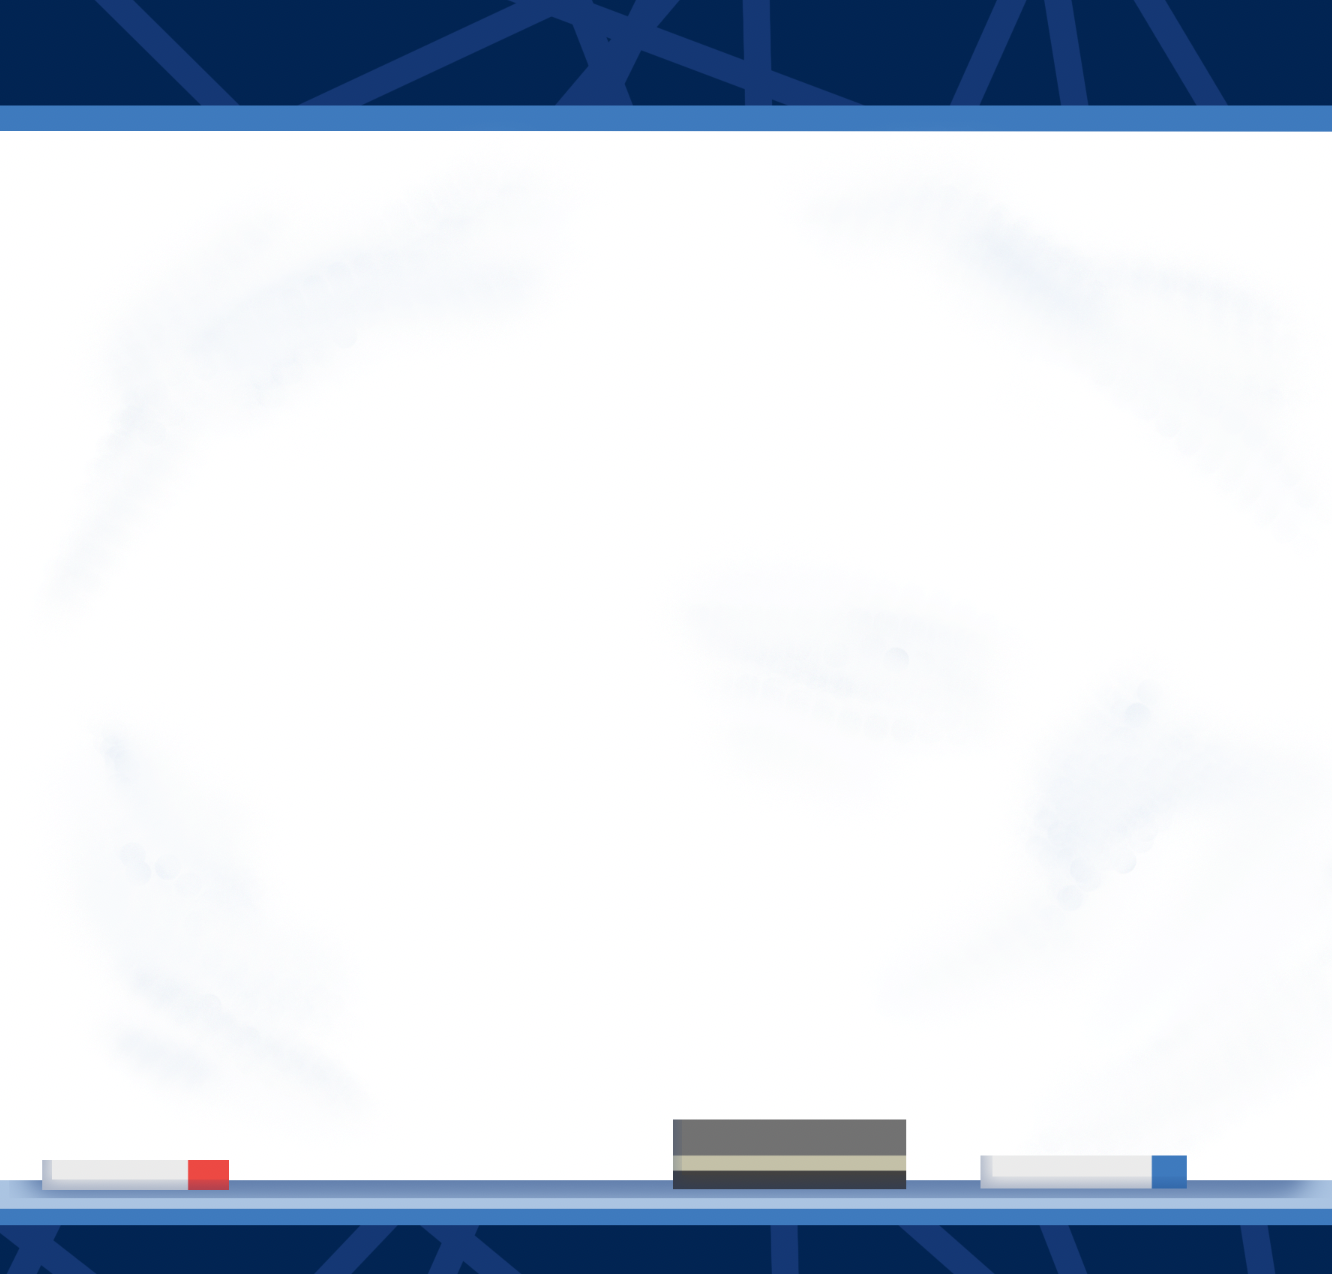
\includegraphics[width=0.9\textwidth, angle=0]{Meetings/August/08-24-21/1.PNG}
\caption{Template 2}
\label{fig:pic1}
\end{figure}

\begin{figure}[htp]
\centering
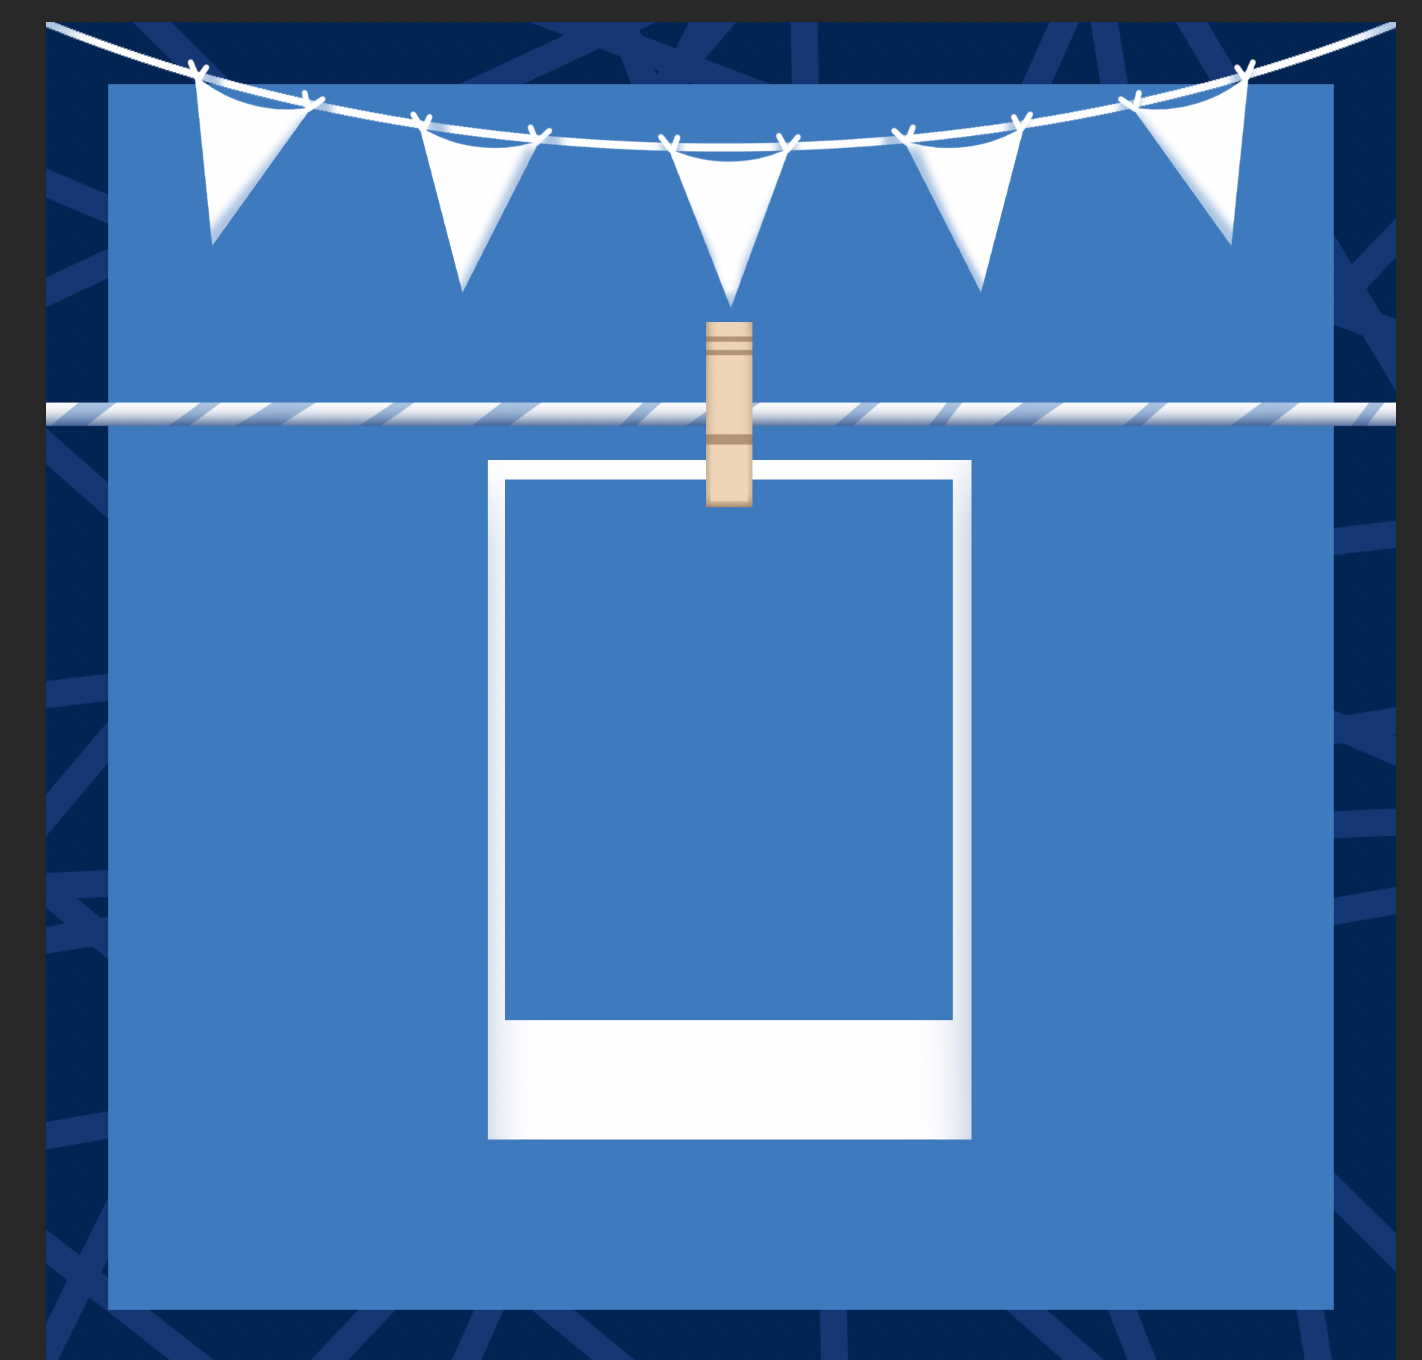
\includegraphics[width=0.9\textwidth, angle=0]{Meetings/August/08-24-21/2.PNG}
\caption{Template 2}
\label{fig:pic2}
\end{figure}

\subsection{Software}
\noindent\hfil\rule{\textwidth}{.4pt}\hfil
\subsubsection{Goals}
\begin{itemize}
    \item Make mecanum work

\end{itemize} 

\noindent\hfil\rule{\textwidth}{.4pt}\hfil

\subsubsection*{Accomplishments}
We decided the controller layout for the drive train. On the left stick, forward and back moves the robot forwards and backwards, while left turns the robot left and right turn the robot right. Even further, we tried to implement vector tracking by utlizing the position of the joystick as a vector, and this would then give us the direction we wanted to go in our robot. This was however quite tedious and we were not able to figure it out in time. Our next steps are to figure out a way to implement Mecanum drive with x, y positions from our joysticks.

\subsection*{Hardware}
\noindent\hfil\rule{\textwidth}{.4pt}\hfil
\subsubsection*{Goals}
\begin{itemize}
    \item Cut remaining parts to intake
    \item Build Intake 

\end{itemize} 

\noindent\hfil\rule{\textwidth}{.4pt}\hfil

\subsubsection*{Accomplishments}
Before this meeting we printed all of the necessary parts and bought all of the needed materials to build the intake. This meant that we were much more prepared and only had to find a few of the vex parts before we could start building. Because we wanted to expand our members’ knowledge in all aspects, one of our hardware members worked alongside one of our sophomore members, who is less experienced with hardware. When we had gathered all of the parts, we started by screwing together the wooden frame of the intake, then added the vex motor and bearings (image 1). When all of the parts were attached, we put the rubber band intake together and attached it to the rest of the intake (image 2 and image 3). 

Unfortunately, we didn't have the correct wire to connect the vex motor to the rev hub, so we couldn’t test the intake being powered, but we turned the motor shaft by hand and tested that way. This gave us a basic idea of what would work. We saw that the intake could reliably collect both blocks and balls, but we noticed that the rubber band part of the intake wasn’t moving up and down in the slots as freely as we had expected. The slots that we put in the sides of the intake were meant to replace a coaxial arm, while making the mechanism small and compact. These slots would allow the rubber band or sweeper part of the intake, as well as the bearing they rest on, to move up and down freely when intaking different sized game elements. We found that the intake plate  had too much friction with the bearings that connected the rubber band roller to the rest of the intake. While brainstorming ideas to make it slide smoother, we came up with the idea of using teflon tape, a type of tape that has a slick surface. We plan on putting teflon tape between the bearing blocks and the intake plate with the slots in it (image4). We were able to put tape on one of the bearings, but we will have to continue in the next meeting. 

\begin{figure}[ht]
\centering
\begin{minipage}[b]{.50\textwidth}
  \centering
  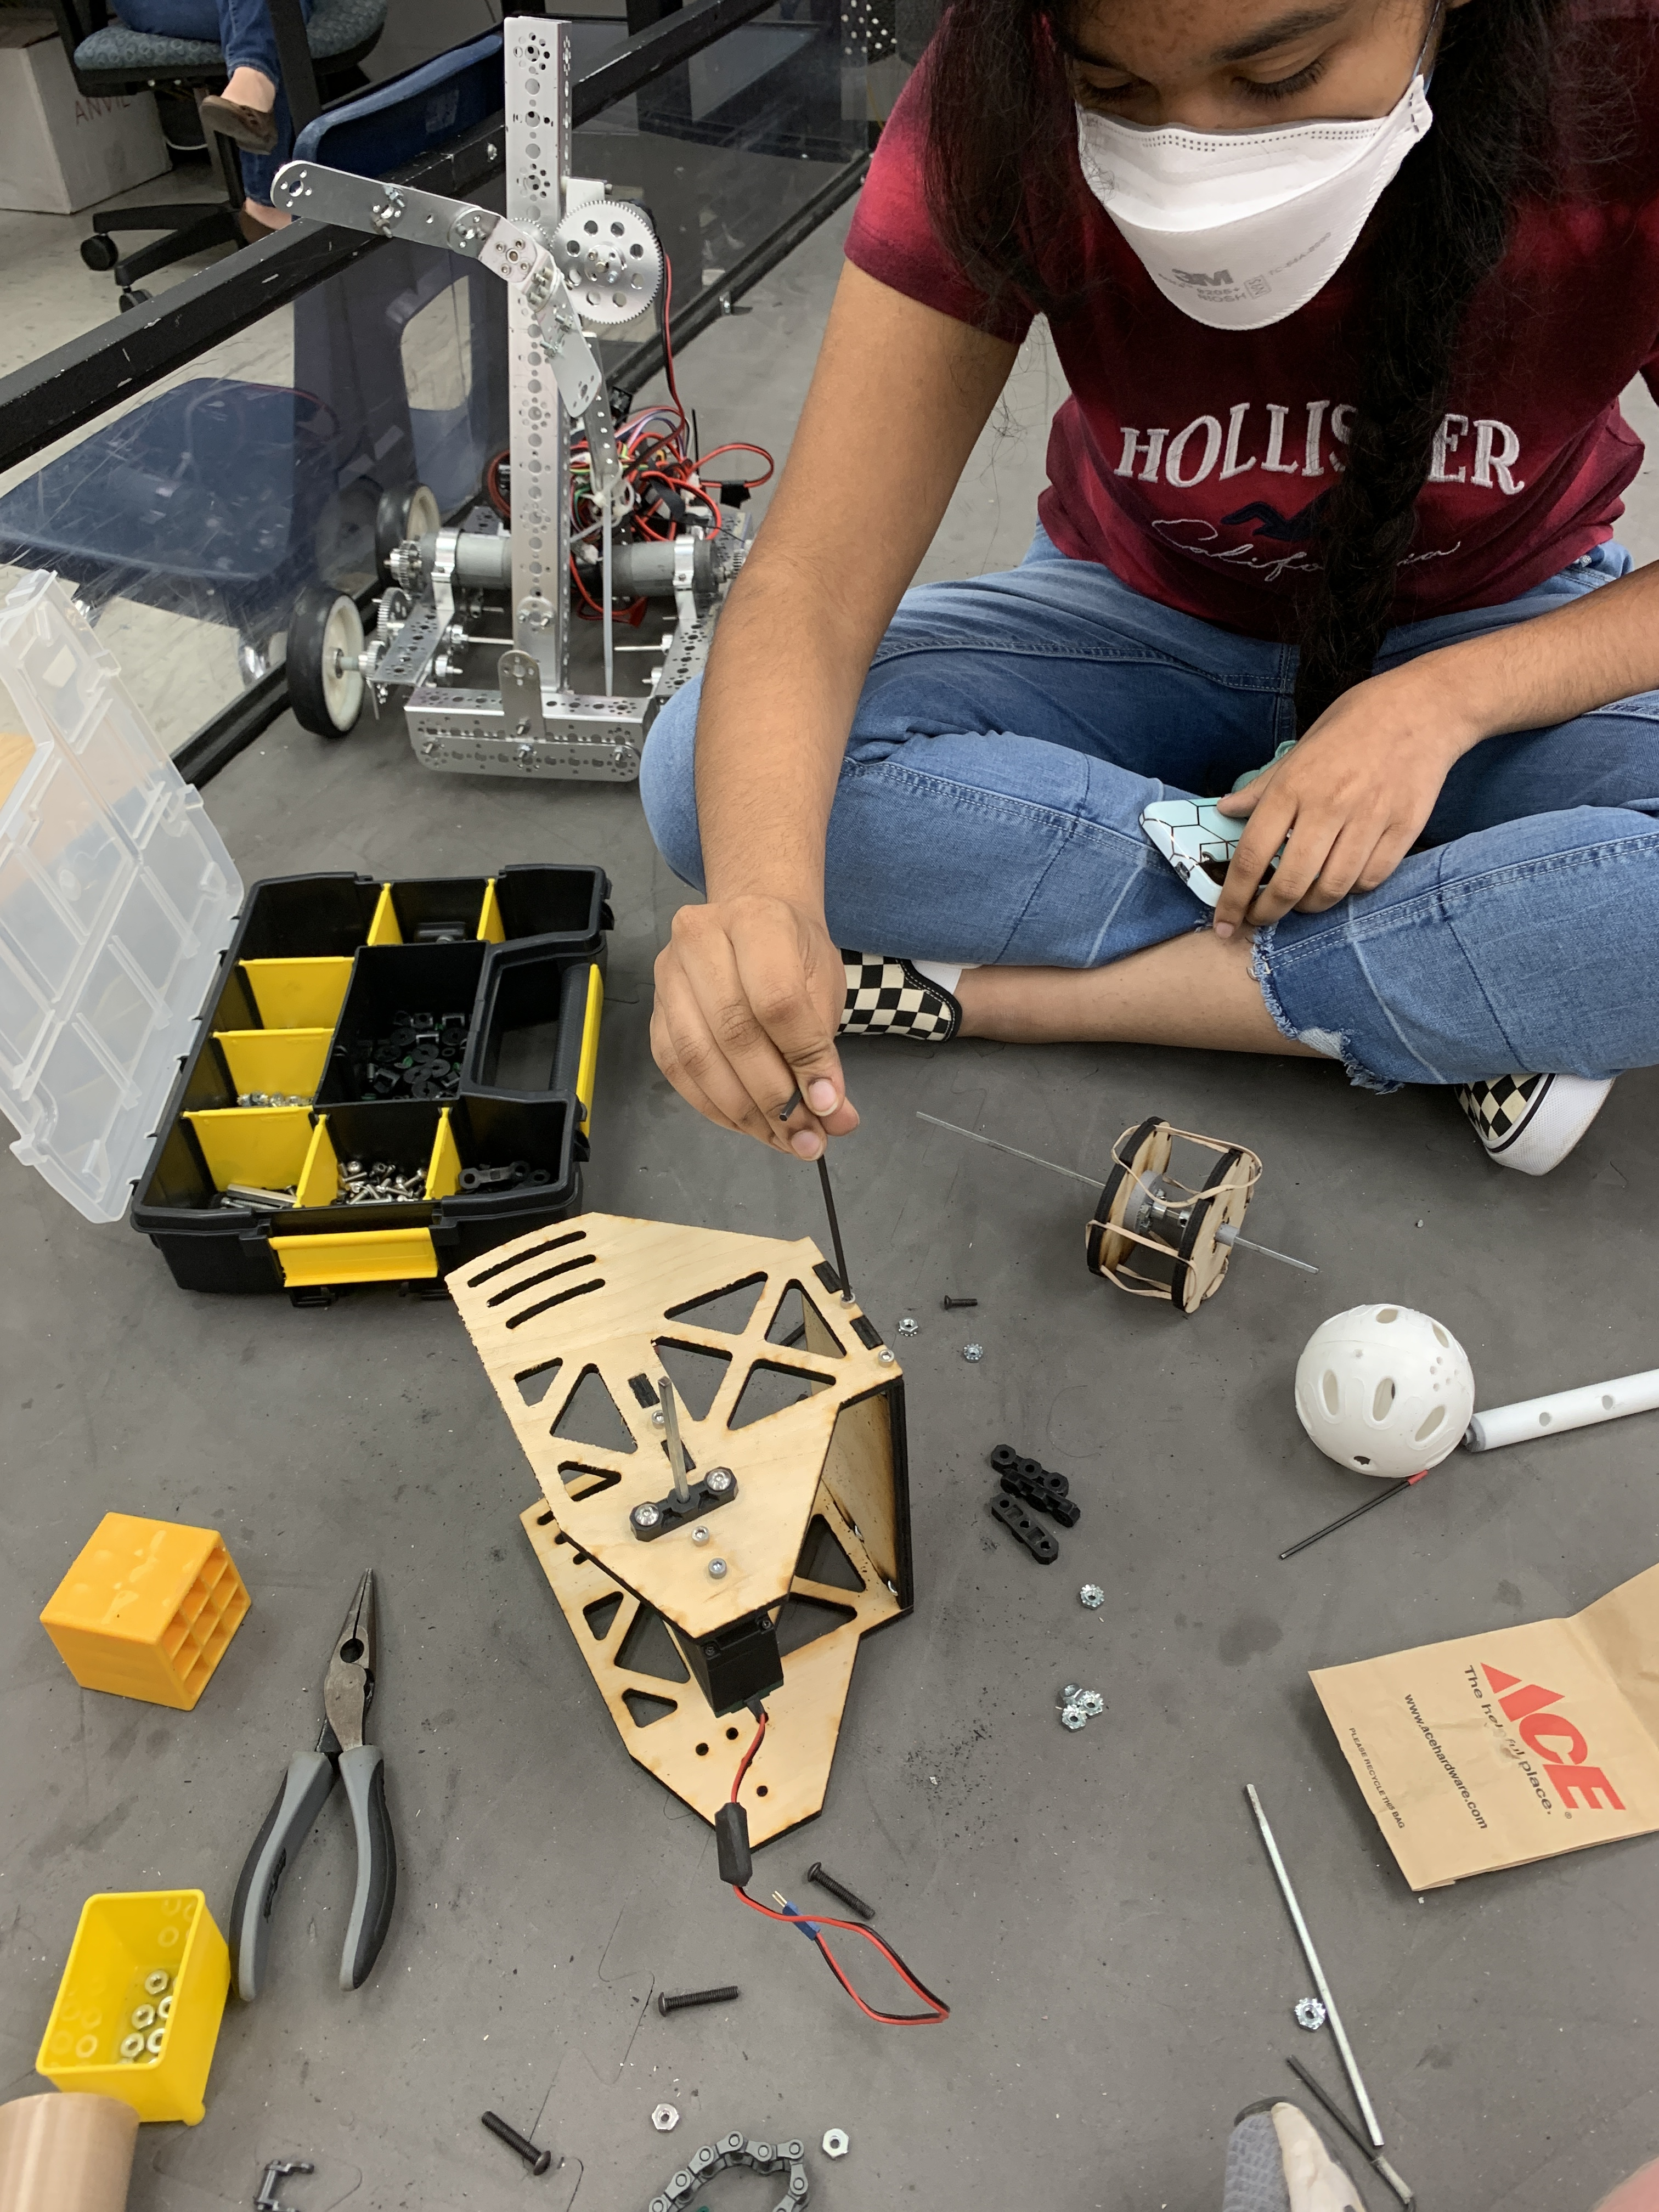
\includegraphics[width=0.8\textwidth]{Meetings/August/08-24-21/8-24-21_Hardware_Image1 - Nathan Forrer.JPG}
  \caption{Anouska working on our prototype}
  \label{fig:pic1}
\end{minipage}%
\hfill%
\begin{minipage}[b]{.50\textwidth}
  \centering
  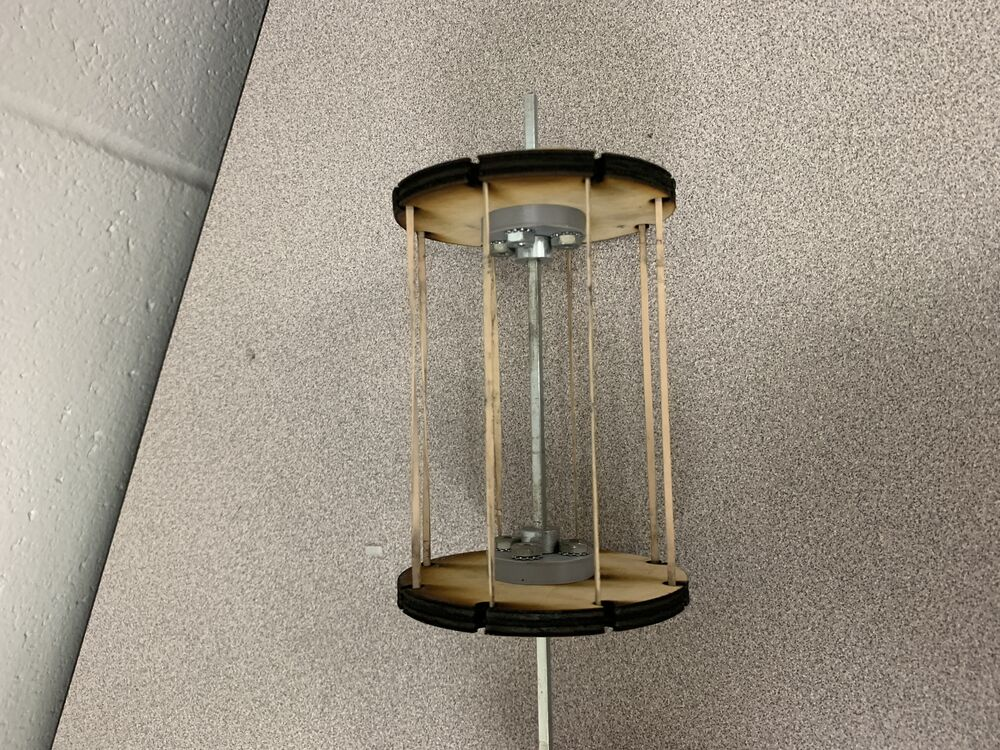
\includegraphics[width=0.8\textwidth]{Meetings/August/08-24-21/8-24-21_Hardware_Image2 - Nathan Forrer.JPG}
  \caption{Intake with rubber bands}
  \label{fig:pic2}
\end{minipage}
\end{figure}

\begin{figure}[ht]
\centering
\begin{minipage}[b]{.50\textwidth}
  \centering
  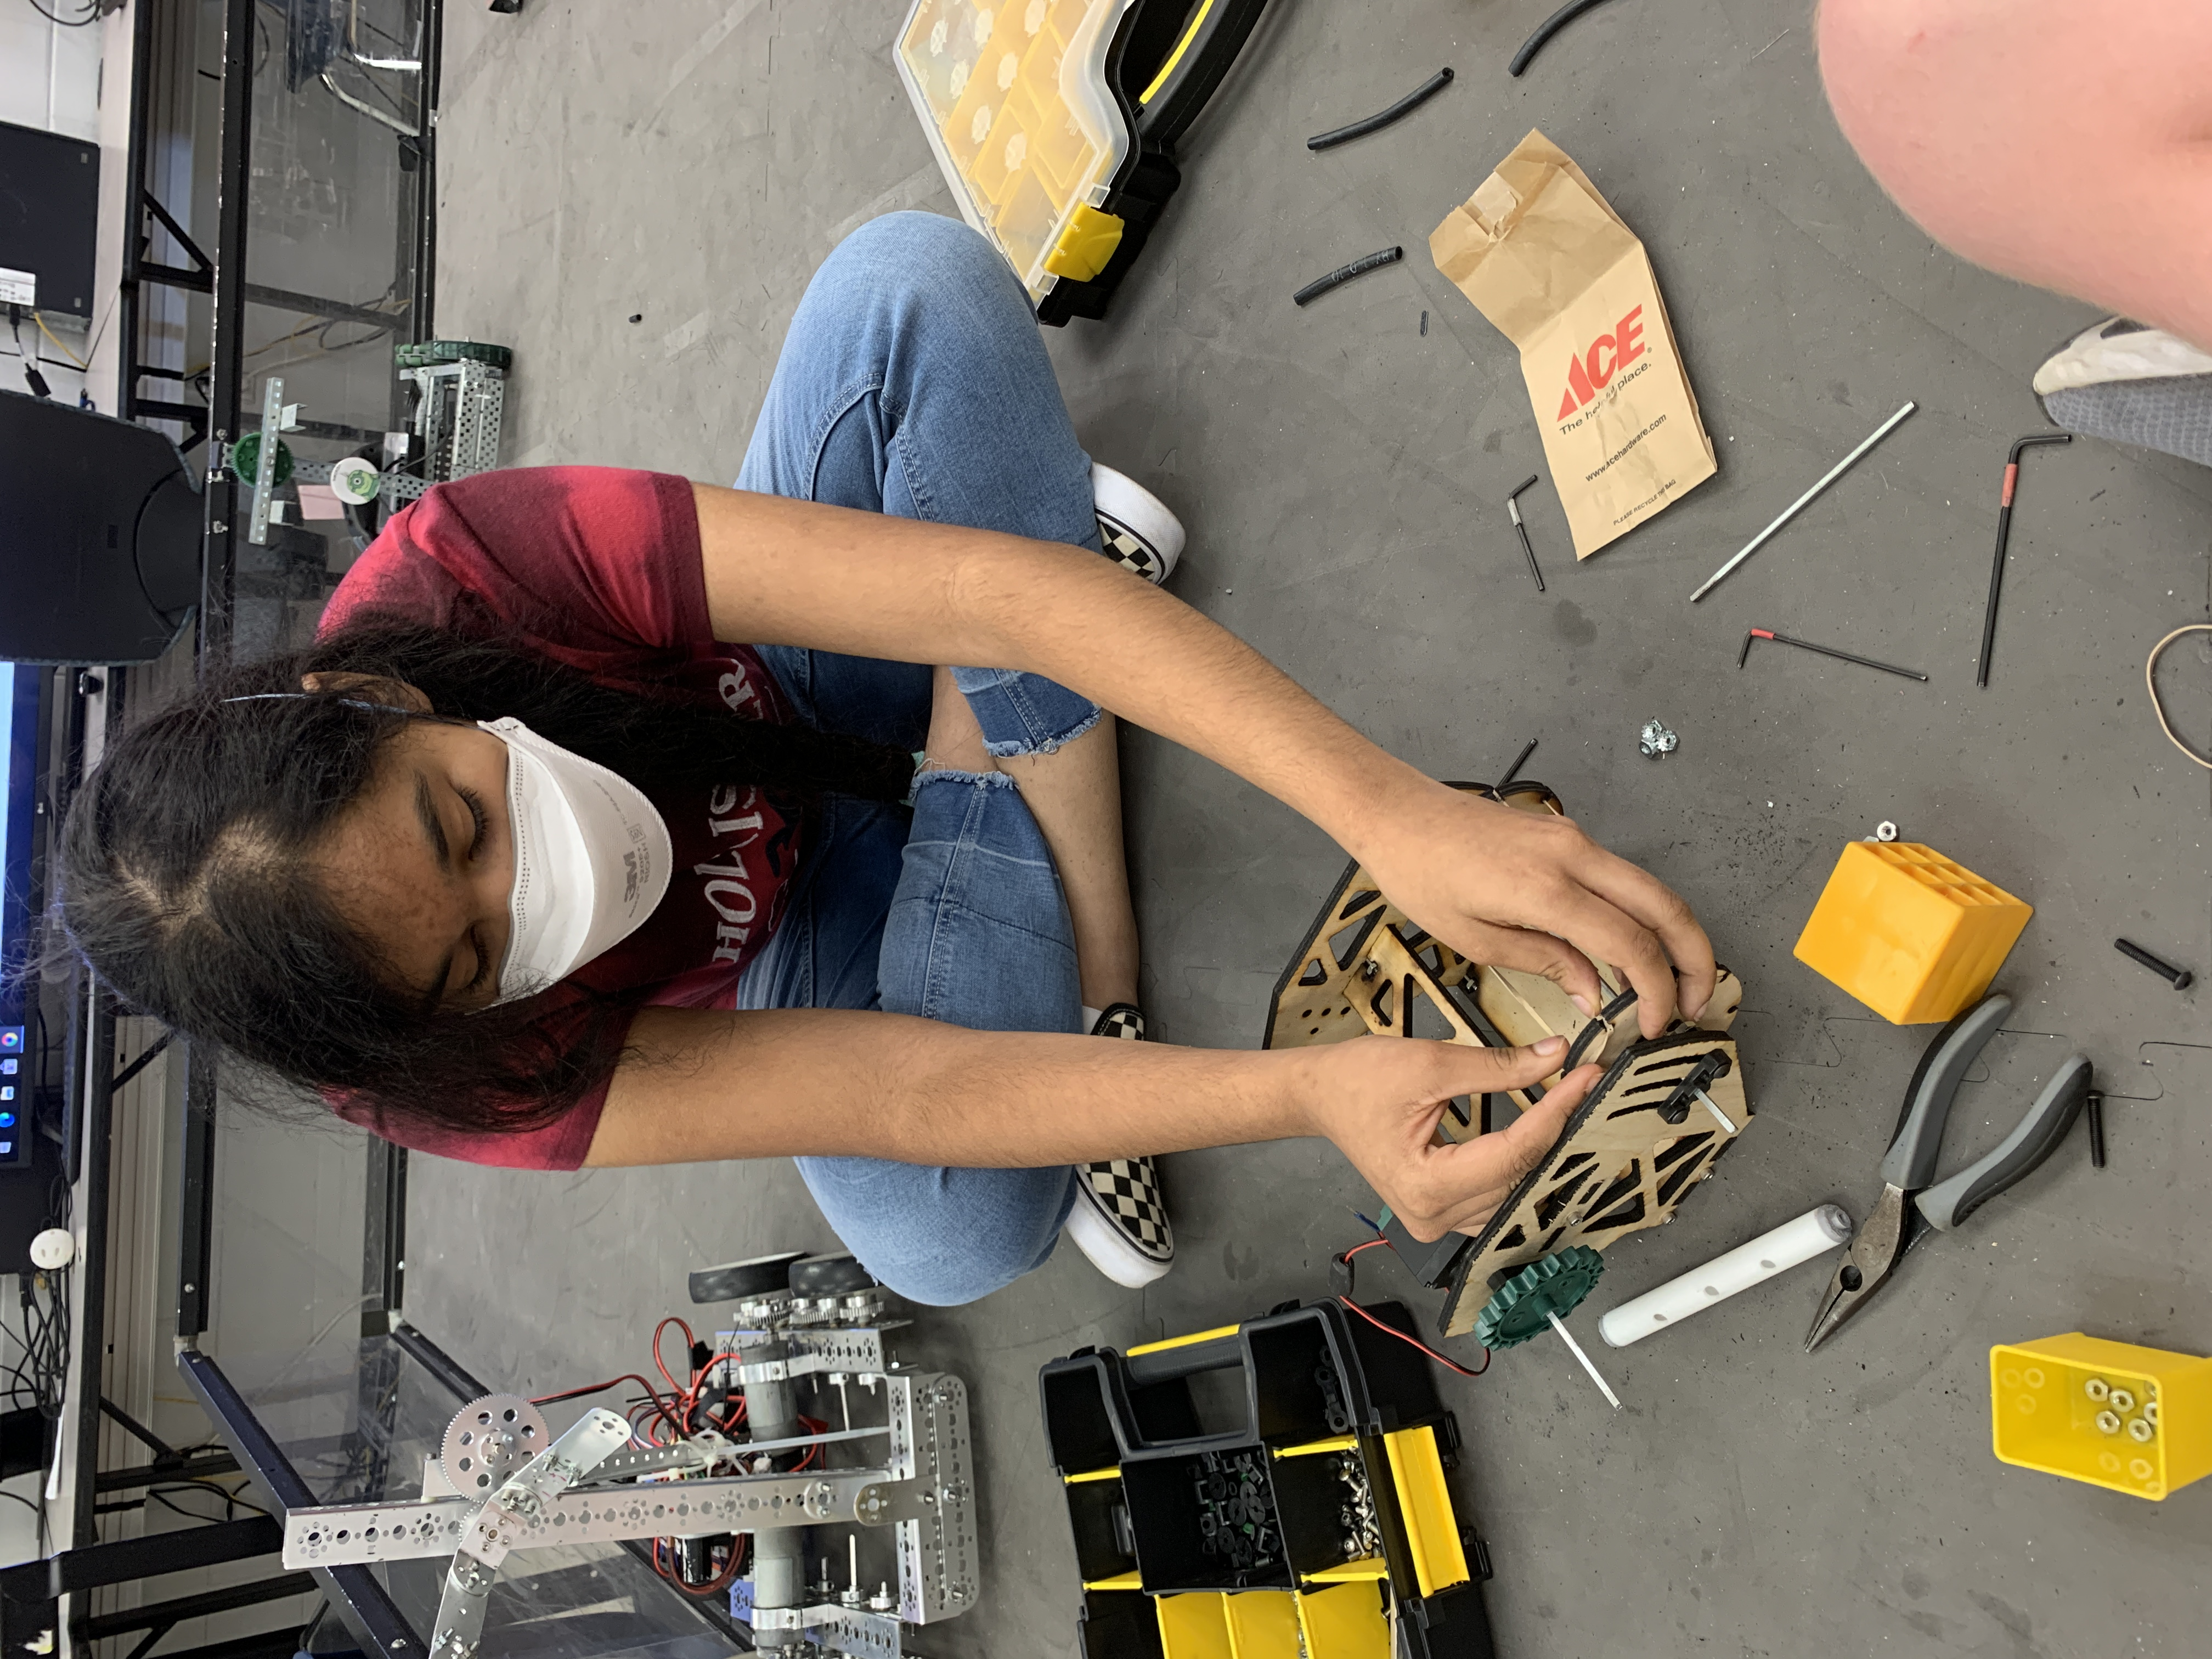
\includegraphics[width=0.8\textwidth]{Meetings/August/08-24-21/8-24-21_Hardware_Image3 - Nathan Forrer.JPG}
  \caption{Building Intake}
  \label{fig:pic3}
\end{minipage}%
\hfill%
\begin{minipage}[b]{.50\textwidth}
  \centering
  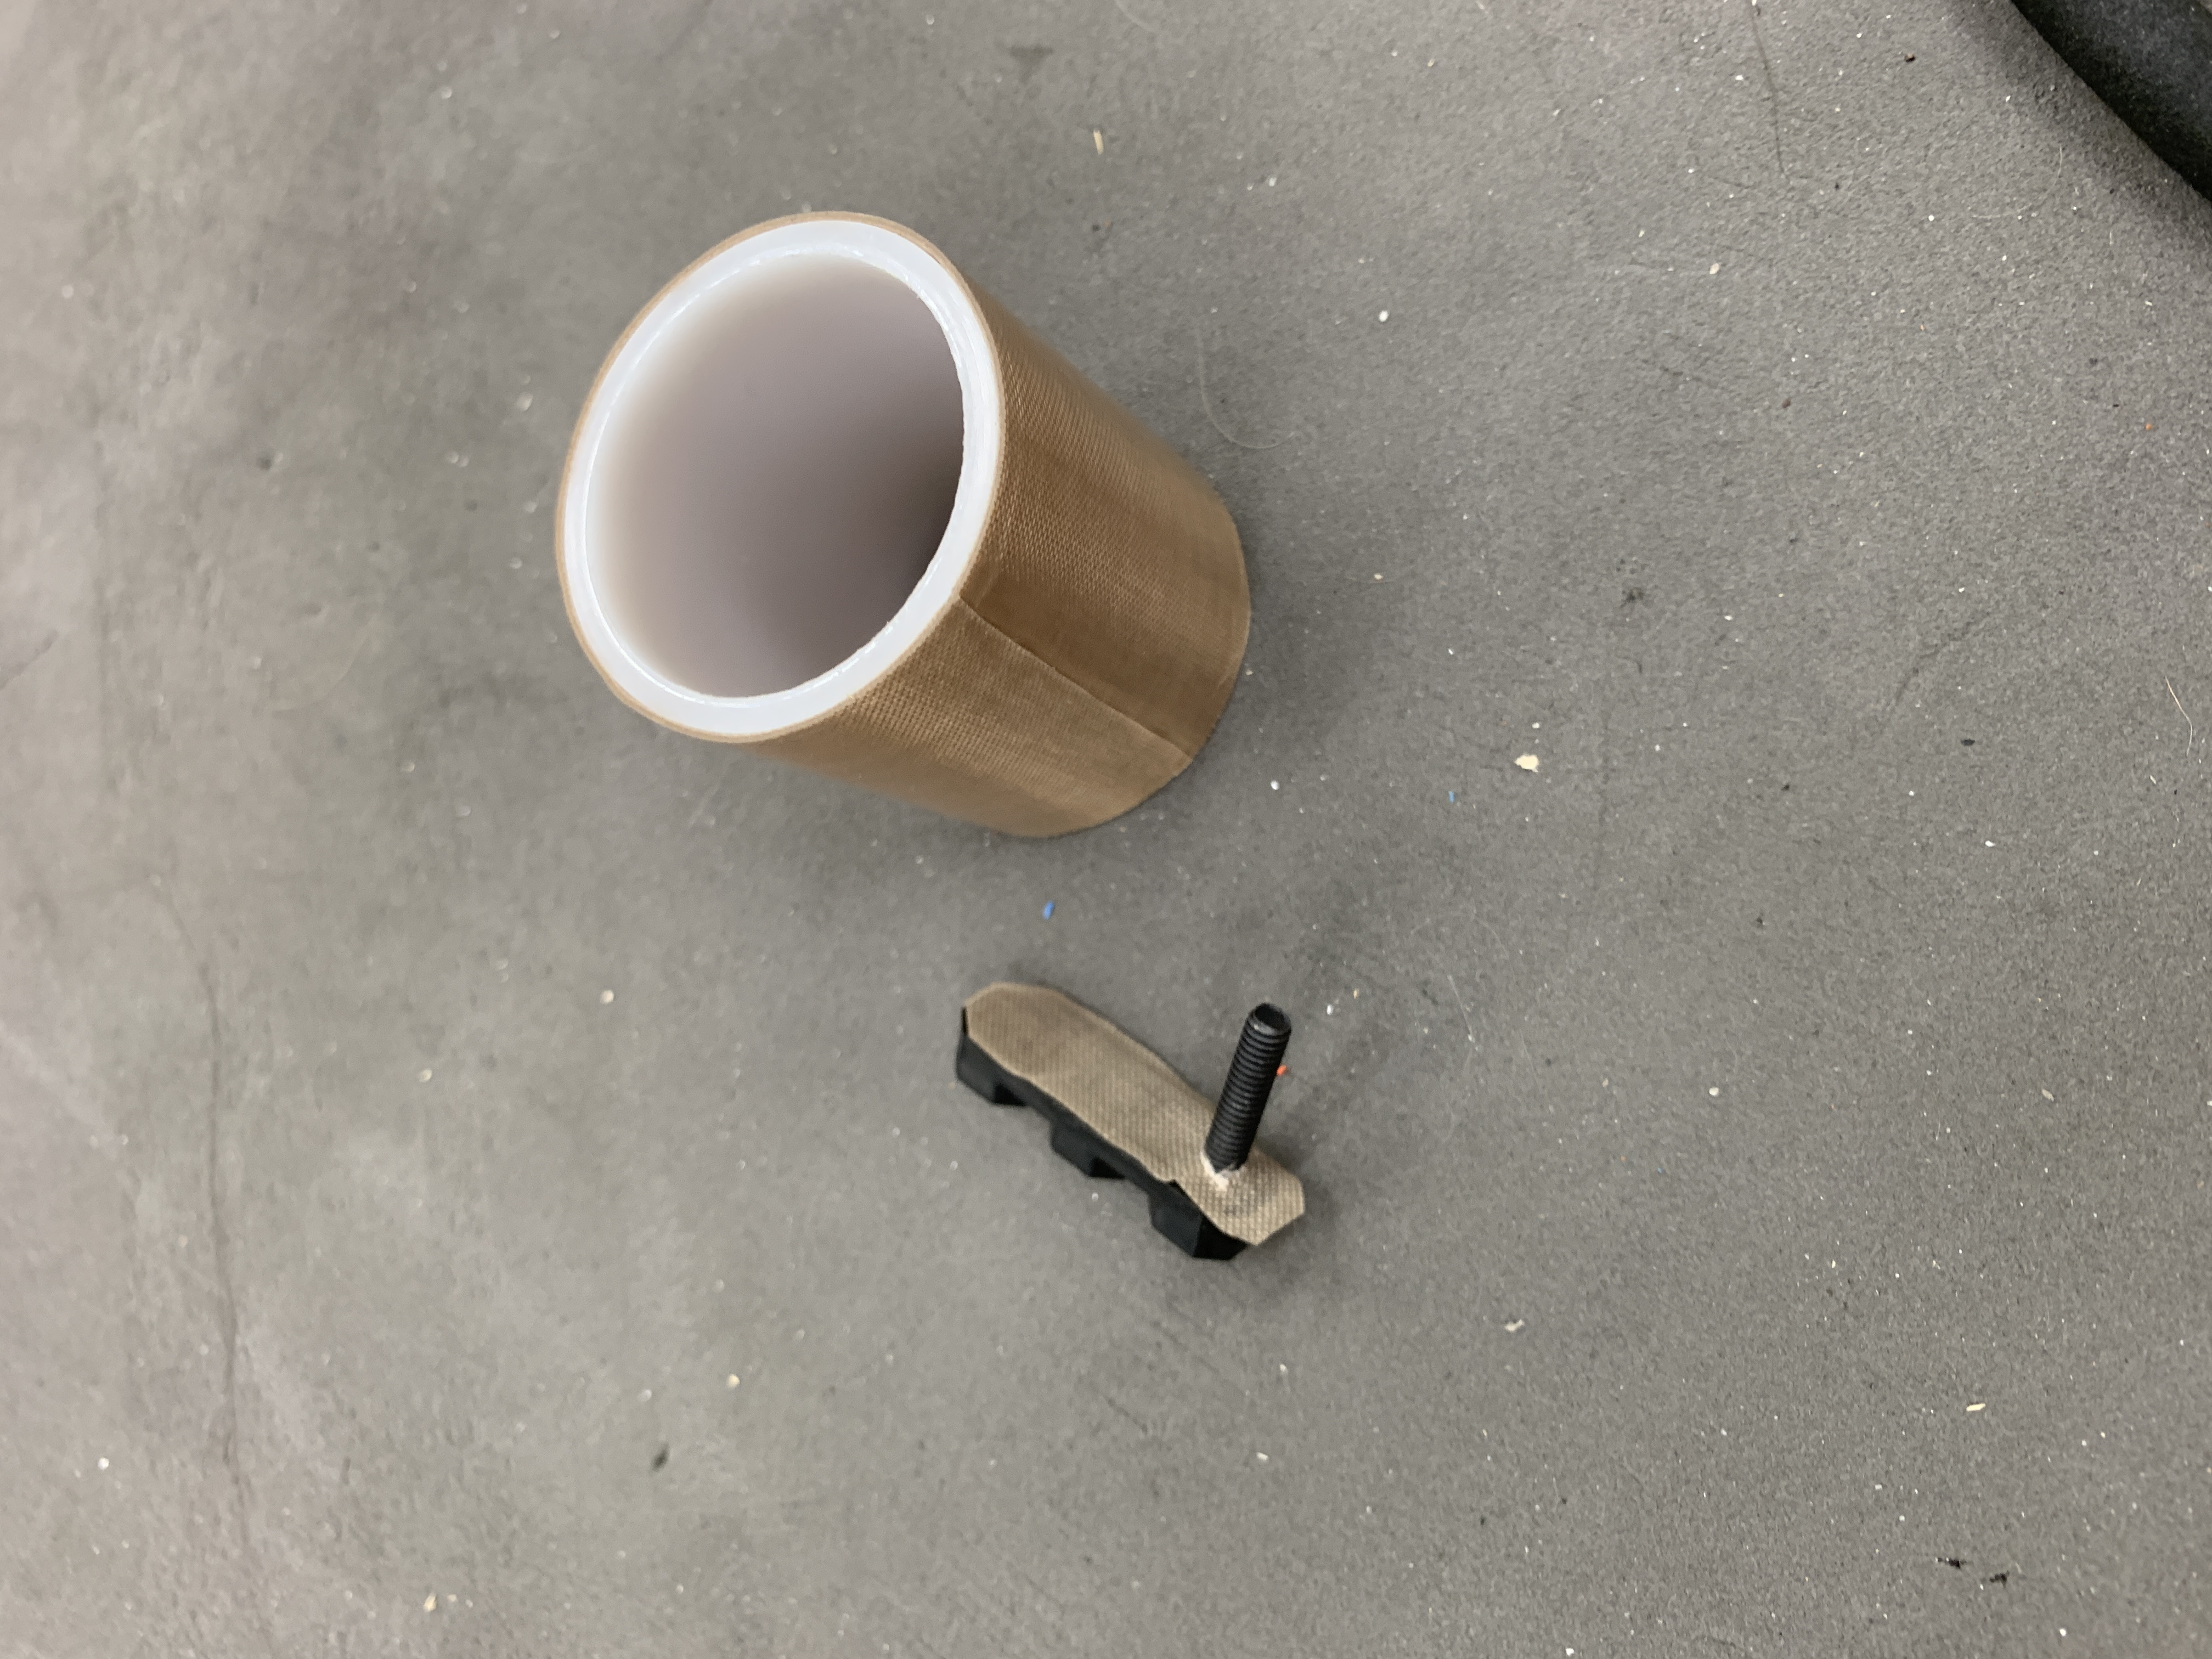
\includegraphics[width=0.8\textwidth]{Meetings/August/08-24-21/8-24-21_Hardware_Image4 - Nathan Forrer.JPG}
  \caption{Bearing Mount}
  \label{fig:pic4}
\end{minipage}
\end{figure}